\subsection{Previsão do tempo}

% http://people.math.aau.dk/~jm/courses/PhD06StocSim/Chapters2.4.5.pdf
% ex 2.1 e 2.2

\begin{questions}
\question{
\begin{description}
\item[Clima em Belo Horizonte]. Muitos belo-horizontinos acreditam que a melhor previsão 
para o tempo de amanhã é permanecer como está hoje. Assumindo-se que esta hipótese esteja
correta, podemos modelar o tempo como uma cadeia de Markov. Para simplificar, vamos 
assumir que existam apenas dois estados: `sol' e `chuva'. Se o preditor ingenuo dos 
belo-horizontinos está correto 75\% das vezes (independente do tempo de hoje ser `sol'
ou `chuva'), então podemos modelar o tempo de Belo Horizonte como uma cadeia de Markov
com dois estados $\mathcal{S}=\{s_1, s_2\}$ ($s_1 = \text{`sol'}$ e $s_1 = \text{`chuva'}$).
\item[Clima do Rio de Janeiro]. No caso de Belo Horizonte, existe uma simetria perfeita entre
`sol' e `chuva', de forma que 75\% das vezes o clima de amanhã será igual ao de hoje,
independente de como esteja o clima hoje. Este modelo pode ser realístico para Belo Horizonte,
que é uma cidade localizada no interior do continente, entretanto, para o Rio de Janeiro, uma cidade litorânea,
tempo de `sol' é muito mais comum. Suponha então que, para o Rio, a probabilidade de ter 
`sol' amanhã, dado que hoje é um dia de `sol', é de 50\%. Se hoje estiver com `chuva', então
a probabilidade de que amanhã faça `sol' é de 90\%.
\end{description}
Para ambos modelos de previsão de tempo (Belo Horizonte e Rio de Janeiro) faça o que se pede
abaixo.

\begin{parts}
\part Em ambos casos, podemos escrever uma matriz de transição para o modelo de previsão do tempo.
Esta matriz será da forma
\begin{equation}
P = 
\begin{pmatrix}
\alpha & 1 - \alpha \\
1 - \beta & \beta
\end{pmatrix} . \nonumber
\end{equation}
Qual é o valor de $\alpha$ e $\beta$ para cada um dos dois modelos?
Represente a cadeia de Markov através de um diagrama de transição.


\part Em ambos casos a cadeia de Markov é invariante no tempo, possuindo assim
uma distribuição estacionária $\mathbf{\mu} = [\mu_1, \ \mu_2]$. Calcule
$\mu_1$ e $\mu_2$. 
%(Dica: encontre a equação para $\mu_1$ e $\mu_2$ em função
%de $\alpha$ e $\beta$; substitua os valores após encontrar as expressões.) 


\part Calcule a taxa de entropia para os dois modelos dados acima.
\end{parts}
}

\begin{solution}
\begin{parts}
\part 
  \begin{description}
  \item[Belo Horizonte]: $\alpha = \beta = 0.75$.
  \item[Rio de Janeiro]: $\alpha = 0.5$, $\beta = 0.1$.
  \end{description}
  \begin{center}
     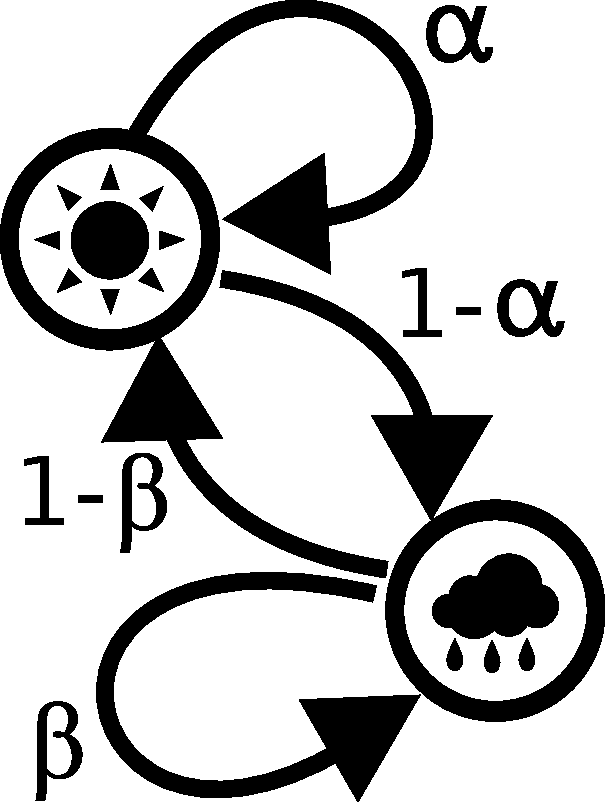
\includegraphics[width=0.15\textwidth]{../images/sunrain.pdf}
  \end{center}

\part
  \begin{equation}
  \mu P = \mu
  \end{equation}

  \begin{equation}
  \begin{pmatrix}
  \mu_1 & \mu_2
  \end{pmatrix}
  \begin{pmatrix}
  \alpha & 1 - \alpha \\
  1 - \beta & \beta
  \end{pmatrix}
  =
  \begin{pmatrix}
  \mu_1 & \mu_2
  \end{pmatrix}
  \end{equation}

  temos então
  \begin{equation}
  \begin{cases}
  \mu_1 \alpha + \mu_2 (1 - \beta) = \mu_1 \\
  \mu_1 (1 - \alpha) + \mu_2 \beta = \mu_2 \\
  \mu_1 + \mu_2 = 1
  \end{cases} 
  \end{equation}
  e assim concluímos que
  \begin{equation}
  \mu_1 = \frac{1 - \beta}{2 - (\alpha + \beta)} \quad \text{ e } \quad \mu_2 = \frac{1 - \alpha}{2 - (\alpha + \beta)} 
  \end{equation}  

  \begin{description}
  \item[Belo Horizonte]: $\mu_1 = \mu_2 = 0.5$.
  \item[Rio de Janeiro]: $\mu_1 = 0.64$, $\mu_2 = 0.36$.
  \end{description}


\part 

  \begin{eqnarray}
   H(\mathcal{X}) &=& \sum_i \mu_i \left[ - \sum_j p_{ij} \log p_{ij} \right]  \\
        &=& \mu_1 \left[ - \alpha \log \alpha - (1 - \alpha) \log (1 - \alpha) \right] + \mu_2 \left[ - (1 - \beta) \log (1 - \beta) - \beta \log \beta  \right] \\
        &=& \mu_1 H(\alpha) + \mu_2 H(\beta) \\
        &=& \frac{1 - \beta}{2 - (\alpha + \beta)} H(\alpha) +  \frac{1 - \alpha}{2 - (\alpha + \beta)} H(\beta)
  \end{eqnarray}

  \begin{description}
  \item[Belo Horizonte]: $H(\mathcal{X}) = 0.81$ bits.
  \item[Rio de Janeiro]: $H(\mathcal{X}) = 0.81$ bits.
  \end{description}

\begin{lstlisting}[language=Octave]
function H = entropy(p)
if length(p) == 1, p = [p, (1-p)]; end;
H = -sum(p.*log2(p));
endfunction

>> alpha=0.75; beta=0.75;
>> ((1 - beta)/(2 - (alpha+beta)))*entropy(alpha) + ...
((1 - alpha)/(2 - (alpha+beta)))*entropy(beta)
ans =  0.81128
>> alpha=0.5; beta=0.1;
>> ((1 - beta)/(2 - (alpha+beta)))*entropy(alpha) + ...
((1 - alpha)/(2 - (alpha+beta)))*entropy(beta)
ans =  0.81036
\end{lstlisting}


\end{parts}
\end{solution}
\end{questions}
